% =====================================================================
%  DSP391m - Group 5  |  Data Tasks: Collection, Cleaning & Analysis
%  EduGuard: AI-Powered Early Warning and Actionable Recourse System
%
%  Standard Beamer deck (Madrid + beaver). Compile with pdfLaTeX.
%  All charts drawn with pgfplots -> nothing to upload but this .tex.
%  Every number is taken from the project's EDA artifacts
%  (reports/eda_findings.json, reports/tables/*.csv).
% =====================================================================
\documentclass[aspectratio=169,10pt]{beamer}

\usetheme{Madrid}
\usecolortheme{beaver}
\setbeamertemplate{navigation symbols}{}
\setbeamertemplate{caption}{\insertcaption}   % plain captions

\usepackage{iftex}
\ifPDFTeX
  \usepackage[T1]{fontenc}
  \usepackage[utf8]{inputenc}
  \usepackage{lmodern}
\else
  \usepackage{fontspec}   % XeTeX/LuaTeX (Tectonic): set real OpenType fonts
\fi
\ifPDFTeX\usepackage{microtype}\fi
\usepackage{booktabs}
\usepackage{array}
\usepackage{tabularx}
\usepackage{colortbl}
\usepackage{graphicx}
\graphicspath{{../figures/}{figures/}{./}}
\usepackage{tikz}
\usepackage{pgfplots}
\pgfplotsset{compat=1.18}
\usepgfplotslibrary{statistics}
\usetikzlibrary{arrows.meta,positioning}

% ---- colours (matched to the beaver theme) ----
\definecolor{themecol}{HTML}{800000}   % dark red, table headers / at-risk
\definecolor{rowtint}{HTML}{F3E9E9}
\definecolor{cblue}{HTML}{1F5C99}
\definecolor{cgreen}{HTML}{2E7D32}
\definecolor{corange}{HTML}{E08214}
\definecolor{cgrey}{HTML}{9E9E9E}

% ---- helpers ----
\newcolumntype{Y}{>{\raggedright\arraybackslash}X}
\newcommand{\hc}[1]{{\bfseries\color{white}#1}}
\newcommand{\tcode}[1]{{\ttfamily #1}}
% one-line italic "takeaway" under a table/chart
\newcommand{\takeaway}[1]{\vspace{2pt}\par{\footnotesize\itshape\textcolor{themecol}{$\Rightarrow$\,}#1}}

\AtBeginSection[]{%
  \begin{frame}{Outline}
    \tableofcontents[currentsection]
  \end{frame}
}

% ---------------------------------------------------------------- meta
\title[Data Tasks]{Data Tasks: Collection, Cleaning \& Analysis}
\subtitle{EduGuard: AI-Powered Early Warning and Actionable Recourse System for Students}
\author[Group 5 -- DSP391m]{Group 5 -- DSP391m}
\institute[FPT University]{FPT University}
\date[DSP391m 2026]{Data Science Capstone (DSP391m) \textbullet{} Report 2}

\begin{document}

\frame{\titlepage}

\begin{frame}{Table of Contents}
  \tableofcontents
\end{frame}

% =====================================================================
\section{Required Data for the Study}
% =====================================================================

\begin{frame}{Data Requirements $\to$ OULAD Sources}
  {\footnotesize
  \setlength{\tabcolsep}{5pt}\renewcommand{\arraystretch}{1.3}
  \begin{tabularx}{\textwidth}{@{}>{\raggedright\arraybackslash}p{3.2cm} Y >{\raggedright\arraybackslash}p{4.1cm}@{}}
    \toprule
    \rowcolor{themecol}\hc{Requirement} & \hc{Why required} & \hc{OULAD source}\\
    \midrule
    Binary at-risk label & Prediction target (all RQs) & \tcode{studentInfo.final\_result}\\
    \rowcolor{rowtint}
    Time-stamped engagement & Checkpoint features (RQ1/2) & \tcode{studentVle} ($\sim$10.6M), \tcode{vle}\\
    Academic performance & Early score signals & \tcode{studentAssessment}, \tcode{assessments}\\
    \rowcolor{rowtint}
    Demographic context & Covariates + fairness & \tcode{studentInfo}, \tcode{studentRegistration}\\
    Course timeline & Date $\to$ progress \% & \tcode{courses} (module length)\\
    \bottomrule
  \end{tabularx}}
  \takeaway{Grain = one row per (student, module, presentation): \textbf{32,593} rows, \textbf{28,785} students, \textbf{22} module-presentations.}
\end{frame}

\begin{frame}{OULAD Composition (7 Relational Tables)}
  {\footnotesize
  \setlength{\tabcolsep}{6pt}\renewcommand{\arraystretch}{1.3}
  \begin{tabularx}{\textwidth}{@{}>{\ttfamily}l Y r c@{}}
    \toprule
    \rowcolor{themecol}\hc{Table} & \hc{Content} & \hc{Rows} & \hc{Time?}\\
    \midrule
    studentInfo         & Demographics + \tcode{final\_result} & 32,593 & no\\
    \rowcolor{rowtint}
    studentRegistration & Registration / withdrawal dates & 32,593 & part\\
    studentVle          & Daily clickstream interactions & 10,655,280 & \textbf{yes}\\
    \rowcolor{rowtint}
    studentAssessment   & Submission dates + scores & $\sim$173,912 & \textbf{yes}\\
    assessments         & Type, weight, deadline & $\sim$206 & part\\
    \rowcolor{rowtint}
    vle                 & Catalogue of activity types & $\sim$6,364 & no\\
    courses             & Module length (days) & 22 & no\\
    \bottomrule
  \end{tabularx}}
  \takeaway{The two date columns -- \tcode{studentVle.date}, \tcode{studentAssessment.date\_submitted} -- enable every time-aware cut.}
\end{frame}

\begin{frame}{Working at Scale -- Understanding 10.6M Rows with ClickHouse}
  \begin{columns}[T]
    \begin{column}{0.50\textwidth}
      \footnotesize\textbf{The problem -- you cannot eyeball it}
      \begin{itemize}\setlength\itemsep{0.25em}
        \item \tcode{studentVle} $=$ \alert{10,655,280} rows / \alert{433\,MB}: too big for Excel; reloading it in pandas \emph{per question} costs GBs of RAM.
        \item \textbf{Method:} \tcode{clickhouse-local} -- one binary, no server, runs SQL straight on CSV/Parquet. Data stays on disk; we push the query down.
      \end{itemize}
      \vspace{2pt}
      \textbf{The type-inference trap}
      \begin{itemize}\setlength\itemsep{0.25em}
        \item Quoted CSV $\Rightarrow$ every column read as \tcode{String}; \tcode{max(date)} returns \alert{"99"} (string compare, ``99''$>$``269'').
        \item Declare the schema $\Rightarrow$ true range \tcode{date} \alert{$-25\to269$}.
      \end{itemize}
    \end{column}
    \begin{column}{0.50\textwidth}
      {\footnotesize
      \setlength{\tabcolsep}{6pt}\renewcommand{\arraystretch}{1.3}
      \begin{tabularx}{\textwidth}{@{}l r r@{}}
        \toprule
        \rowcolor{themecol}\hc{} & \hc{Size} & \hc{\tcode{count()}}\\
        \midrule
        CSV      & 433\,MB  & $\approx$14.6\,s\\
        \rowcolor{rowtint}
        Parquet  & 22.9\,MB & $\approx$0.55\,s\\
        \midrule
        \textbf{Gain} & \alert{$\sim$20$\times$} & \alert{$\sim$26$\times$}\\
        \bottomrule
      \end{tabularx}}
      \vspace{3pt}\par\footnotesize\textbf{Profiled in one pass}
      \begin{itemize}\setlength\itemsep{0.2em}
        \item \alert{26,074} students actually click (of 28,785).
        \item per-event clicks: median 2, skew \alert{122}.
        \item \tcode{total\_clicks} skew \alert{3.0} $\Rightarrow$ motivates log1p.
      \end{itemize}
    \end{column}
  \end{columns}
  \takeaway{Push SQL to the data: 10.6M rows understood in $<$1\,s, and \textbf{every number on these slides is reproducible} (\tcode{notebooks/00\_data\_understanding}).}
\end{frame}

\begin{frame}{Target Variable \& Class Balance}
  \begin{columns}[T]
    \begin{column}{0.50\textwidth}
      {\scriptsize
      \setlength{\tabcolsep}{5pt}\renewcommand{\arraystretch}{1.25}
      \begin{tabularx}{\textwidth}{@{}l r Y@{}}
        \toprule
        \rowcolor{themecol}\hc{\texttt{final\_result}} & \hc{Count} & \hc{Label}\\
        \midrule
        Pass        & 12,361 & not-at-risk (0)\\
        \rowcolor{rowtint}
        Distinction &  3,024 & not-at-risk (0)\\
        Withdrawn   & 10,156 & \textbf{at-risk (1)}\\
        \rowcolor{rowtint}
        Fail        &  7,052 & \textbf{at-risk (1)}\\
        \bottomrule
      \end{tabularx}}
      \vspace{4pt}\par
      \scriptsize
      \tcode{at\_risk = \{Fail, Withdrawn\}}\\[2pt]
      At-risk \textbf{52.8\%} \textbullet{} imbalance ratio \textbf{1.12} (mild).\\
      Metric focus: \textbf{PR-AUC} + \textbf{recall} on at-risk.
    \end{column}
    \begin{column}{0.50\textwidth}
      \centering
      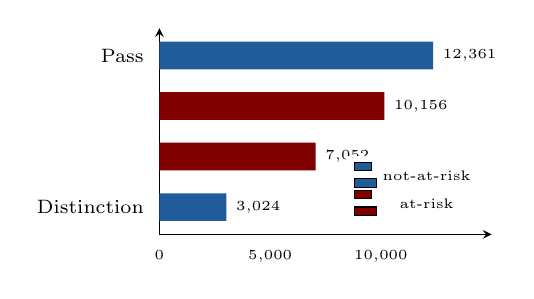
\begin{tikzpicture}
        \begin{axis}[
          width=5.8cm,height=4.2cm,
          xbar,xmin=0,xmax=15000,
          bar width=10pt,bar shift=0pt,
          symbolic y coords={Distinction,Fail,Withdrawn,Pass},
          ytick=data,yticklabel style={font=\scriptsize},
          nodes near coords,every node near coord/.append style={font=\tiny},
          xtick={0,5000,10000},xticklabel style={font=\tiny},
          scaled x ticks=false,
          axis lines=left,tick style={draw=none},
          enlarge y limits=0.18,
          legend style={font=\tiny,at={(0.98,0.05)},anchor=south east,draw=none},
        ]
        \addplot[fill=cblue,draw=none] coordinates {(12361,Pass) (3024,Distinction)};
        \addplot[fill=themecol,draw=none] coordinates {(10156,Withdrawn) (7052,Fail)};
        \legend{not-at-risk,at-risk}
        \end{axis}
      \end{tikzpicture}\\
      {\scriptsize\itshape Withdrawn is the largest single class.}
    \end{column}
  \end{columns}
\end{frame}

% =====================================================================
\section{Data Collection Method}
% =====================================================================

\begin{frame}{Choosing a Data Source}
  {\footnotesize
  \setlength{\tabcolsep}{6pt}\renewcommand{\arraystretch}{1.3}
  \begin{tabularx}{\textwidth}{@{}>{\raggedright\arraybackslash}p{3.8cm} c c c >{\columncolor{rowtint}}c@{}}
    \toprule
    \rowcolor{themecol}\hc{Criterion} & \hc{Internal DB} & \hc{API} & \hc{Scraping} & \hc{Public}\\
    \midrule
    Immediate availability      & Low  & Medium & Medium    & \textbf{High}\\
    Already anonymised          & No   & No     & No        & \textbf{Yes}\\
    Reproducibility             & Low  & Low    & Very low  & \textbf{High}\\
    Comparability w/ prior work & Low  & Low    & Low       & \textbf{High}\\
    Ethical / legal complexity  & High & Medium & High      & \textbf{Low (CC)}\\
    \bottomrule
  \end{tabularx}}
  \takeaway{OULAD is \textbf{public secondary data}: we trade collection-design control for reproducibility \& comparability with the base studies (Adnan 2021; Tomasevic 2020).}
\end{frame}

\begin{frame}{Why OULAD -- and License \& Ethics}
  \begin{columns}[t,onlytextwidth]
    \begin{column}{0.47\textwidth}
      \begin{block}{Fit to the project}
        \scriptsize
        \begin{itemize}\setlength\itemsep{0.25em}
          \item Publicly downloadable -- reproducible by anyone.
          \item All 3 feature groups: demographics, VLE, assessments.
          \item Labelled \tcode{final\_result} $\to$ \tcode{at\_risk}.
          \item Same dataset as the base studies $\Rightarrow$ direct comparison.
          \item Static snapshot -- identical file for everyone.
        \end{itemize}
      \end{block}
    \end{column}
    \hfill
    \begin{column}{0.47\textwidth}
      \begin{block}{License \& ethics}
        \scriptsize
        \begin{itemize}\setlength\itemsep{0.25em}
          \item \textbf{CC-BY 4.0} -- reuse with attribution only.
          \item Anonymised at source: no IDs; region-level; banded age \& IMD.
          \item No re-identification; no external linkage.
          \item Raw CSVs read-only + md5 verification.
          \item Cite Kuzilek et al.\ (2017), \emph{Scientific Data}.
        \end{itemize}
      \end{block}
    \end{column}
  \end{columns}
\end{frame}

% =====================================================================
\section{Data Cleaning Strategy}
% =====================================================================

\begin{frame}{Data Quality Profile -- Where Are the Defects?}
  {\scriptsize
  \setlength{\tabcolsep}{5pt}\renewcommand{\arraystretch}{1.3}
  \begin{tabularx}{\textwidth}{@{}>{\ttfamily}l r r >{\raggedright\arraybackslash}p{2.2cm} Y@{}}
    \toprule
    \rowcolor{themecol}\hc{Column} & \hc{\#Missing} & \hc{\%} & \hc{Mechanism} & \hc{Handling (where)}\\
    \midrule
    date\_unregistration & 22,521 & 69.1 & structural & dropped -- not a feature\\
    \rowcolor{rowtint}
    imd\_band            & 1,111  & 3.41 & MAR / MCAR & $\to$ \texttt{"Unknown"} (ordinal rank 0)\\
    date\_registration   & 45     & 0.14 & MCAR       & $\to$ \textbf{train} median\\
    score\_*\_to\_date (3)& by design & --  & MNAR      & $\to$ 0 + \texttt{not\_submitted} flag\\
    \rowcolor{rowtint}
    all 29 other columns & 0      & 0.0  & --         & none needed\\
    \bottomrule
  \end{tabularx}}
  \takeaway{Duplicates on the composite key: \textbf{0}. After imputation: \textbf{0 NaN} in every feature column (train \& test).}
\end{frame}

\begin{frame}{Missing Values -- Method \& Justification}
  {\scriptsize
  \setlength{\tabcolsep}{5pt}\renewcommand{\arraystretch}{1.35}
  \begin{tabularx}{\textwidth}{@{}>{\ttfamily}l >{\raggedright\arraybackslash}p{3.1cm} Y@{}}
    \toprule
    \rowcolor{themecol}\hc{Variable} & \hc{Strategy} & \hc{Why this, not deletion/mean}\\
    \midrule
    imd\_band & $\to$ \texttt{"Unknown"} category & Keeps the ordinal scale; never fabricates a deprivation value.\\
    \rowcolor{rowtint}
    score\_*\_to\_date & $\to$ 0 + \texttt{not\_submitted} & A missing score \emph{is} a signal (nothing handed in yet); the flag stops 0 being read as a real zero score.\\
    date\_registration & $\to$ \textbf{train} median & Only 45 rows, MCAR; train-only fit avoids leakage.\\
    \rowcolor{rowtint}
    date\_unregistration & dropped & 69.1\% missing is structural; imputing a fake date has no meaning.\\
    \bottomrule
  \end{tabularx}}
  \takeaway{All statistics are learned on the \textbf{training fold only}, then applied to test (no leakage).}
\end{frame}

\begin{frame}{Outliers -- Severe Right-Skew in the Clickstream}
  \begin{columns}[T]
    \begin{column}{0.52\textwidth}
      \centering
      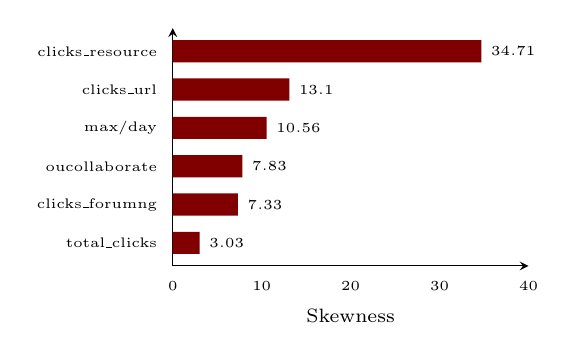
\begin{tikzpicture}
        \begin{axis}[
          width=6.1cm,height=4.6cm,
          xbar,xmin=0,xmax=40,ymin=0.4,ymax=6.6,
          bar width=8pt,
          ytick={1,2,3,4,5,6},yticklabel style={font=\tiny},
          yticklabels={total\_clicks,clicks\_forumng,oucollaborate,max/day,clicks\_url,clicks\_resource},
          nodes near coords,every node near coord/.append style={font=\tiny},
          xtick={0,10,20,30,40},xticklabel style={font=\tiny},
          xlabel={\scriptsize Skewness},axis lines=left,tick style={draw=none},
        ]
        \addplot[fill=themecol,draw=none] coordinates {
          (3.03,1) (7.33,2) (7.83,3) (10.56,4) (13.10,5) (34.71,6)};
        \end{axis}
      \end{tikzpicture}
    \end{column}
    \begin{column}{0.48\textwidth}
      \footnotesize\textbf{Evidence (IQR rule, train)}
      \begin{itemize}\setlength\itemsep{0.3em}
        \item \tcode{clicks\_resource}: skew \alert{34.7}, kurtosis \alert{2125}, max \alert{5,147} vs median 19.
        \item \tcode{max\_clicks\_single\_day}: max \alert{6,988} vs median 74.
        \item A symmetric variable has skew $\approx 0$; here it is huge $\Rightarrow$ long right tail.
      \end{itemize}
      \takeaway{Untreated, these extremes dominate gradients/distances and inflate variance.}
    \end{column}
  \end{columns}
\end{frame}

\begin{frame}{Outliers -- Method, Choice \& Evaluation}
  {\scriptsize
  \setlength{\tabcolsep}{5pt}\renewcommand{\arraystretch}{1.3}
  \begin{tabularx}{\textwidth}{@{}>{\raggedright\arraybackslash}p{2.0cm} >{\raggedright\arraybackslash}p{3.6cm} Y@{}}
    \toprule
    \rowcolor{themecol}\hc{Strategy} & \hc{Applied to} & \hc{Why / evaluation}\\
    \midrule
    \tcode{log1p} & all clickstream counts (\tcode{total\_clicks}, \tcode{n\_days\_active}, 8$\times$\tcode{clicks\_*}, \tcode{max\_clicks\_single\_day}) & Compresses the long tail, maps 0$\to$0 (many zero-activity students).\\
    \rowcolor{rowtint}
    winsorise 1\% & \tcode{studied\_credits}, \tcode{num\_of\_prev\_attempts}, \tcode{weighted\_score}, \tcode{days\_since\_last\_activity} & Clips top/bottom 1\%, keeps the rank; safer than log on a score.\\
    none & \tcode{mean\_score\_to\_date}, \tcode{n\_assessments}, \tcode{date\_registration} & IQR upper bound 103 $>$ max 100 $\Rightarrow$ no true outlier.\\
    \bottomrule
  \end{tabularx}}
  \takeaway{\textbf{No row is ever deleted} -- only transformed; thresholds learned per training fold.}
\end{frame}

% =====================================================================
\section{Data Transformation \& Standardisation}
% =====================================================================

\begin{frame}{Variable Typing -- 28 Features, 5 Types}
  {\footnotesize
  \setlength{\tabcolsep}{6pt}\renewcommand{\arraystretch}{1.3}
  \begin{tabularx}{\textwidth}{@{}>{\raggedright\arraybackslash}p{2.0cm} c Y >{\raggedright\arraybackslash}p{3.0cm}@{}}
    \toprule
    \rowcolor{themecol}\hc{Type} & \hc{\#} & \hc{Examples} & \hc{Encoder / scaler}\\
    \midrule
    Numeric   & 19 & clicks, scores, \tcode{studied\_credits} & \tcode{StandardScaler}\\
    \rowcolor{rowtint}
    Ordinal   & 3  & \tcode{highest\_education}, \tcode{imd\_band}, \tcode{age\_band} & \tcode{OrdinalEncoder}\\
    Nominal   & 3  & \tcode{region}, \tcode{code\_module}, \tcode{code\_presentation} & \tcode{OneHotEncoder}\\
    \rowcolor{rowtint}
    Binary    & 2  & \tcode{gender}, \tcode{disability} & \tcode{BinaryEncoder}\\
    Indicator & 1  & \tcode{not\_submitted} & passthrough\\
    \bottomrule
  \end{tabularx}}
  \takeaway{Type drives the transformer: wrong type = lost rank (ordinal) or a false order (nominal).}
\end{frame}

\begin{frame}{Encoding -- Method \& Rationale}
  {\scriptsize
  \setlength{\tabcolsep}{5pt}\renewcommand{\arraystretch}{1.3}
  \begin{tabularx}{\textwidth}{@{}>{\ttfamily}l Y@{}}
    \toprule
    \rowcolor{themecol}\hc{Encoder} & \hc{Key configuration \& why}\\
    \midrule
    OrdinalEncoder & Explicit category order (e.g.\ \tcode{No Formal} $<$ \ldots $<$ \tcode{Post Grad}); \tcode{unknown=-1}. Preserves rank, no dimensionality blow-up.\\
    \rowcolor{rowtint}
    OneHotEncoder  & \tcode{handle\_unknown=ignore}, \tcode{drop=None}. No false order; every category stays visible for SHAP/LIME.\\
    BinaryEncoder  & Fixed map M/Y$\to$1, F/N$\to$0. Deterministic, no fitting needed.\\
    \rowcolor{rowtint}
    passthrough    & \tcode{not\_submitted} already 0/1 from feature engineering.\\
    \bottomrule
  \end{tabularx}}
  \takeaway{\tcode{drop=None} is deliberate: dropping a reference column would hide that category from explanations.}
\end{frame}

\begin{frame}{Standardisation: Before $\to$ After}
  {\footnotesize
  \setlength{\tabcolsep}{6pt}\renewcommand{\arraystretch}{1.35}
  \begin{tabularx}{\textwidth}{@{}>{\raggedright\arraybackslash}p{2.8cm} Y Y@{}}
    \toprule
    \rowcolor{themecol}\hc{Component} & \hc{Before} & \hc{After}\\
    \midrule
    Labels   & class names & binary at-risk = 1 / 0\\
    \rowcolor{rowtint}
    Categorical & text values & numeric (ordinal/one-hot/binary)\\
    Numeric  & raw, skewed, 0--24k & \tcode{log1p}/winsorise + z-score (mean 0, sd 1)\\
    \rowcolor{rowtint}
    Matrix   & 28 mixed-scale cols & \alert{49}-column dense, 0 NaN\\
    Names    & raw & \tcode{snake\_case}, transformer-prefixed\\
    \bottomrule
  \end{tabularx}}
  \takeaway{Scaler fitted on \textbf{train only} (\tcode{scaler.mean\_} from train); test uses \tcode{.transform()} -- never \tcode{.fit\_transform()}.}
\end{frame}

\begin{frame}{Preprocessing Sequence -- Fit on Train Only}
  \begin{columns}[T]
    \begin{column}{0.55\textwidth}
      \centering
      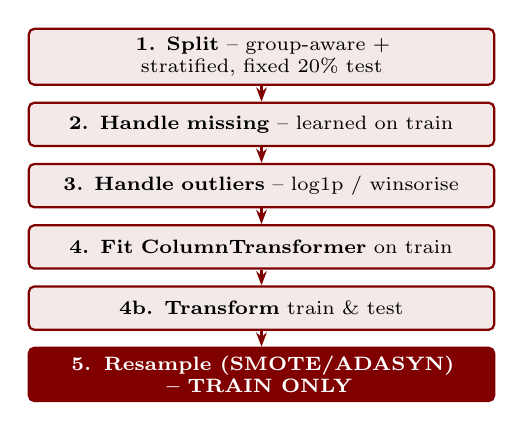
\begin{tikzpicture}[
        box/.style={draw=themecol,line width=0.8pt,rounded corners=2pt,fill=rowtint,
          text width=5.7cm,align=center,font=\scriptsize,inner sep=3pt,minimum height=0.55cm},
        hl/.style={draw=themecol,line width=0.8pt,rounded corners=2pt,fill=themecol,text=white,
          text width=5.7cm,align=center,font=\scriptsize\bfseries,inner sep=3pt,minimum height=0.55cm},
        arr/.style={-{Stealth[length=1.8mm]},themecol,line width=0.8pt}]
        \node[box](a){\textbf{1. Split} -- group-aware + stratified, fixed 20\% test};
        \node[box,below=0.2cm of a](b){\textbf{2. Handle missing} -- learned on train};
        \node[box,below=0.2cm of b](c){\textbf{3. Handle outliers} -- log1p / winsorise};
        \node[box,below=0.2cm of c](d){\textbf{4. Fit ColumnTransformer} on train};
        \node[box,below=0.2cm of d](e){\textbf{4b. Transform} train \& test};
        \node[hl,below=0.2cm of e](f){5. Resample (SMOTE/ADASYN) -- TRAIN ONLY};
        \draw[arr](a)--(b);\draw[arr](b)--(c);\draw[arr](c)--(d);\draw[arr](d)--(e);\draw[arr](e)--(f);
      \end{tikzpicture}
    \end{column}
    \begin{column}{0.45\textwidth}
      \footnotesize\textbf{Anti-leakage reasons}
      \begin{itemize}\setlength\itemsep{0.35em}
        \item Split \alert{first} -- no statistic flows test$\to$train.
        \item Impute/encode/scale \alert{fit on train}, apply to test.
        \item Outlier thresholds per fold; \alert{no rows dropped}.
        \item Resample \alert{train only} -- test keeps real class ratio.
        \item Mirrors the time cut (\tcode{cut\_at\_checkpoint}).
      \end{itemize}
    \end{column}
  \end{columns}
\end{frame}

% =====================================================================
\section{Train/Test Split \& Leakage Control}
% =====================================================================

\begin{frame}{Why the Split Needs Care}
  \begin{columns}[t,onlytextwidth]
    \begin{column}{0.30\textwidth}
      \begin{block}{1. Grouped}\scriptsize A student spans several module-presentations $\Rightarrow$ split by \tcode{id\_student}, else group leakage.\end{block}
    \end{column}
    \hfill
    \begin{column}{0.30\textwidth}
      \begin{block}{2. Imbalanced}\scriptsize At-risk $\approx$52.8\% $\Rightarrow$ \emph{stratify} so the test ratio cannot drift.\end{block}
    \end{column}
    \hfill
    \begin{column}{0.30\textwidth}
      \begin{block}{3. Time-aware}\scriptsize 6 checkpoints share one axis $\Rightarrow$ test set \emph{identical} at each.\end{block}
    \end{column}
  \end{columns}
  \vspace{6pt}
  {\footnotesize
  \setlength{\tabcolsep}{7pt}\renewcommand{\arraystretch}{1.2}
  \begin{tabularx}{\textwidth}{@{}Y Y Y Y Y@{}}
    \rowcolor{themecol}\hc{Train rows} & \hc{Test rows} & \hc{Test students} & \hc{At-risk tr/te} & \hc{Overlap}\\
    \midrule
    26,104 & 6,489 & 5,756 & .530 / .520 & \alert{0}\\
    \bottomrule
  \end{tabularx}}
  \takeaway{Verified on \tcode{master\_raw} (32,593 rows), identical across all six checkpoints.}
\end{frame}

\begin{frame}{Splitting Strategies Compared}
  {\scriptsize
  \setlength{\tabcolsep}{5pt}\renewcommand{\arraystretch}{1.3}
  \begin{tabularx}{\textwidth}{@{}>{\raggedright\arraybackslash}p{2.4cm} Y Y@{}}
    \toprule
    \rowcolor{themecol}\hc{Strategy} & \hc{Pros} & \hc{Cons}\\
    \midrule
    Single hold-out & simple, fast & high variance; one partition\\
    \rowcolor{rowtint}
    k-fold CV & uses all data; lower variance & $k\times$ cost; still seed-dependent\\
    \textbf{Repeated k-fold} & \textbf{robust mean$\pm$std; seed-independent} & highest cost\\
    \rowcolor{rowtint}
    Nested CV & unbiased with tuning & very expensive, complex\\
    \bottomrule
  \end{tabularx}}
  \takeaway{\textbf{Chosen:} fixed 20\% hold-out + \textbf{5-fold $\times$ 5-seed} repeated CV (\tcode{StratifiedGroupKFold}) -- robust yet comparable across checkpoints. Report mean$\pm$std PR-AUC / recall.}
\end{frame}

\begin{frame}{Leakage Prevention -- and It Is Tested}
  \footnotesize\textbf{Three temporal rules (per checkpoint $t$, cutoff $=$ \tcode{round(length$\times t/100$)})}
  \begin{enumerate}\setlength\itemsep{0.25em}
    \item Drop assessment submissions with \tcode{date\_submitted > cutoff}.
    \item Drop VLE interactions with \tcode{date > cutoff} (\tcode{cut\_at\_checkpoint}).
    \item Withdrawn-before-$t$ kept \& labelled at-risk -- low activity is signal, not leakage.
  \end{enumerate}
  \textbf{+ Fit-on-train principle} for every learner (imputers, encoders, scaler, resampler).
  \vspace{4pt}
  \begin{exampleblock}{Verified automatically by \tcode{tests/test\_leakage.py}}
    \centering {\large\bfseries 19 / 19 tests pass}\\[2pt]
    {\scriptsize no record beyond cutoff \textbullet{} counts non-decreasing in $t$ \textbullet{} $t{=}100\%$ keeps all \textbullet{} 0 overlap \textbullet{} ratio preserved \textbullet{} train-only impute/winsorise \textbullet{} no-leak feature allow-list}
  \end{exampleblock}
\end{frame}

\begin{frame}{Time-Aware Checkpoints -- Signal Grows With Time}
  \begin{columns}[T]
    \begin{column}{0.44\textwidth}
      \footnotesize Six checkpoints: \alert{10 / 20 / 40 / 60 / 80 / 100\%}.
      \vspace{3pt}
      \par\textbf{Earliest checkpoint reaching $d\geq0.8$:}
      {\scriptsize
      \setlength{\tabcolsep}{4pt}\renewcommand{\arraystretch}{1.15}
      \begin{tabularx}{\textwidth}{@{}Y r@{}}
        \rowcolor{themecol}\hc{Feature} & \hc{at $t=$}\\
        n\_days\_active, days\_idle & \textbf{10\%}\\
        \rowcolor{rowtint}
        mean\_score / n\_assess / weighted\_score & \textbf{20\%}\\
        total\_clicks         & 60\%\\
      \end{tabularx}}
      \takeaway{\scriptsize Useful signal exists \textbf{early} -- the basis for early intervention.}
    \end{column}
    \begin{column}{0.56\textwidth}
      \centering
      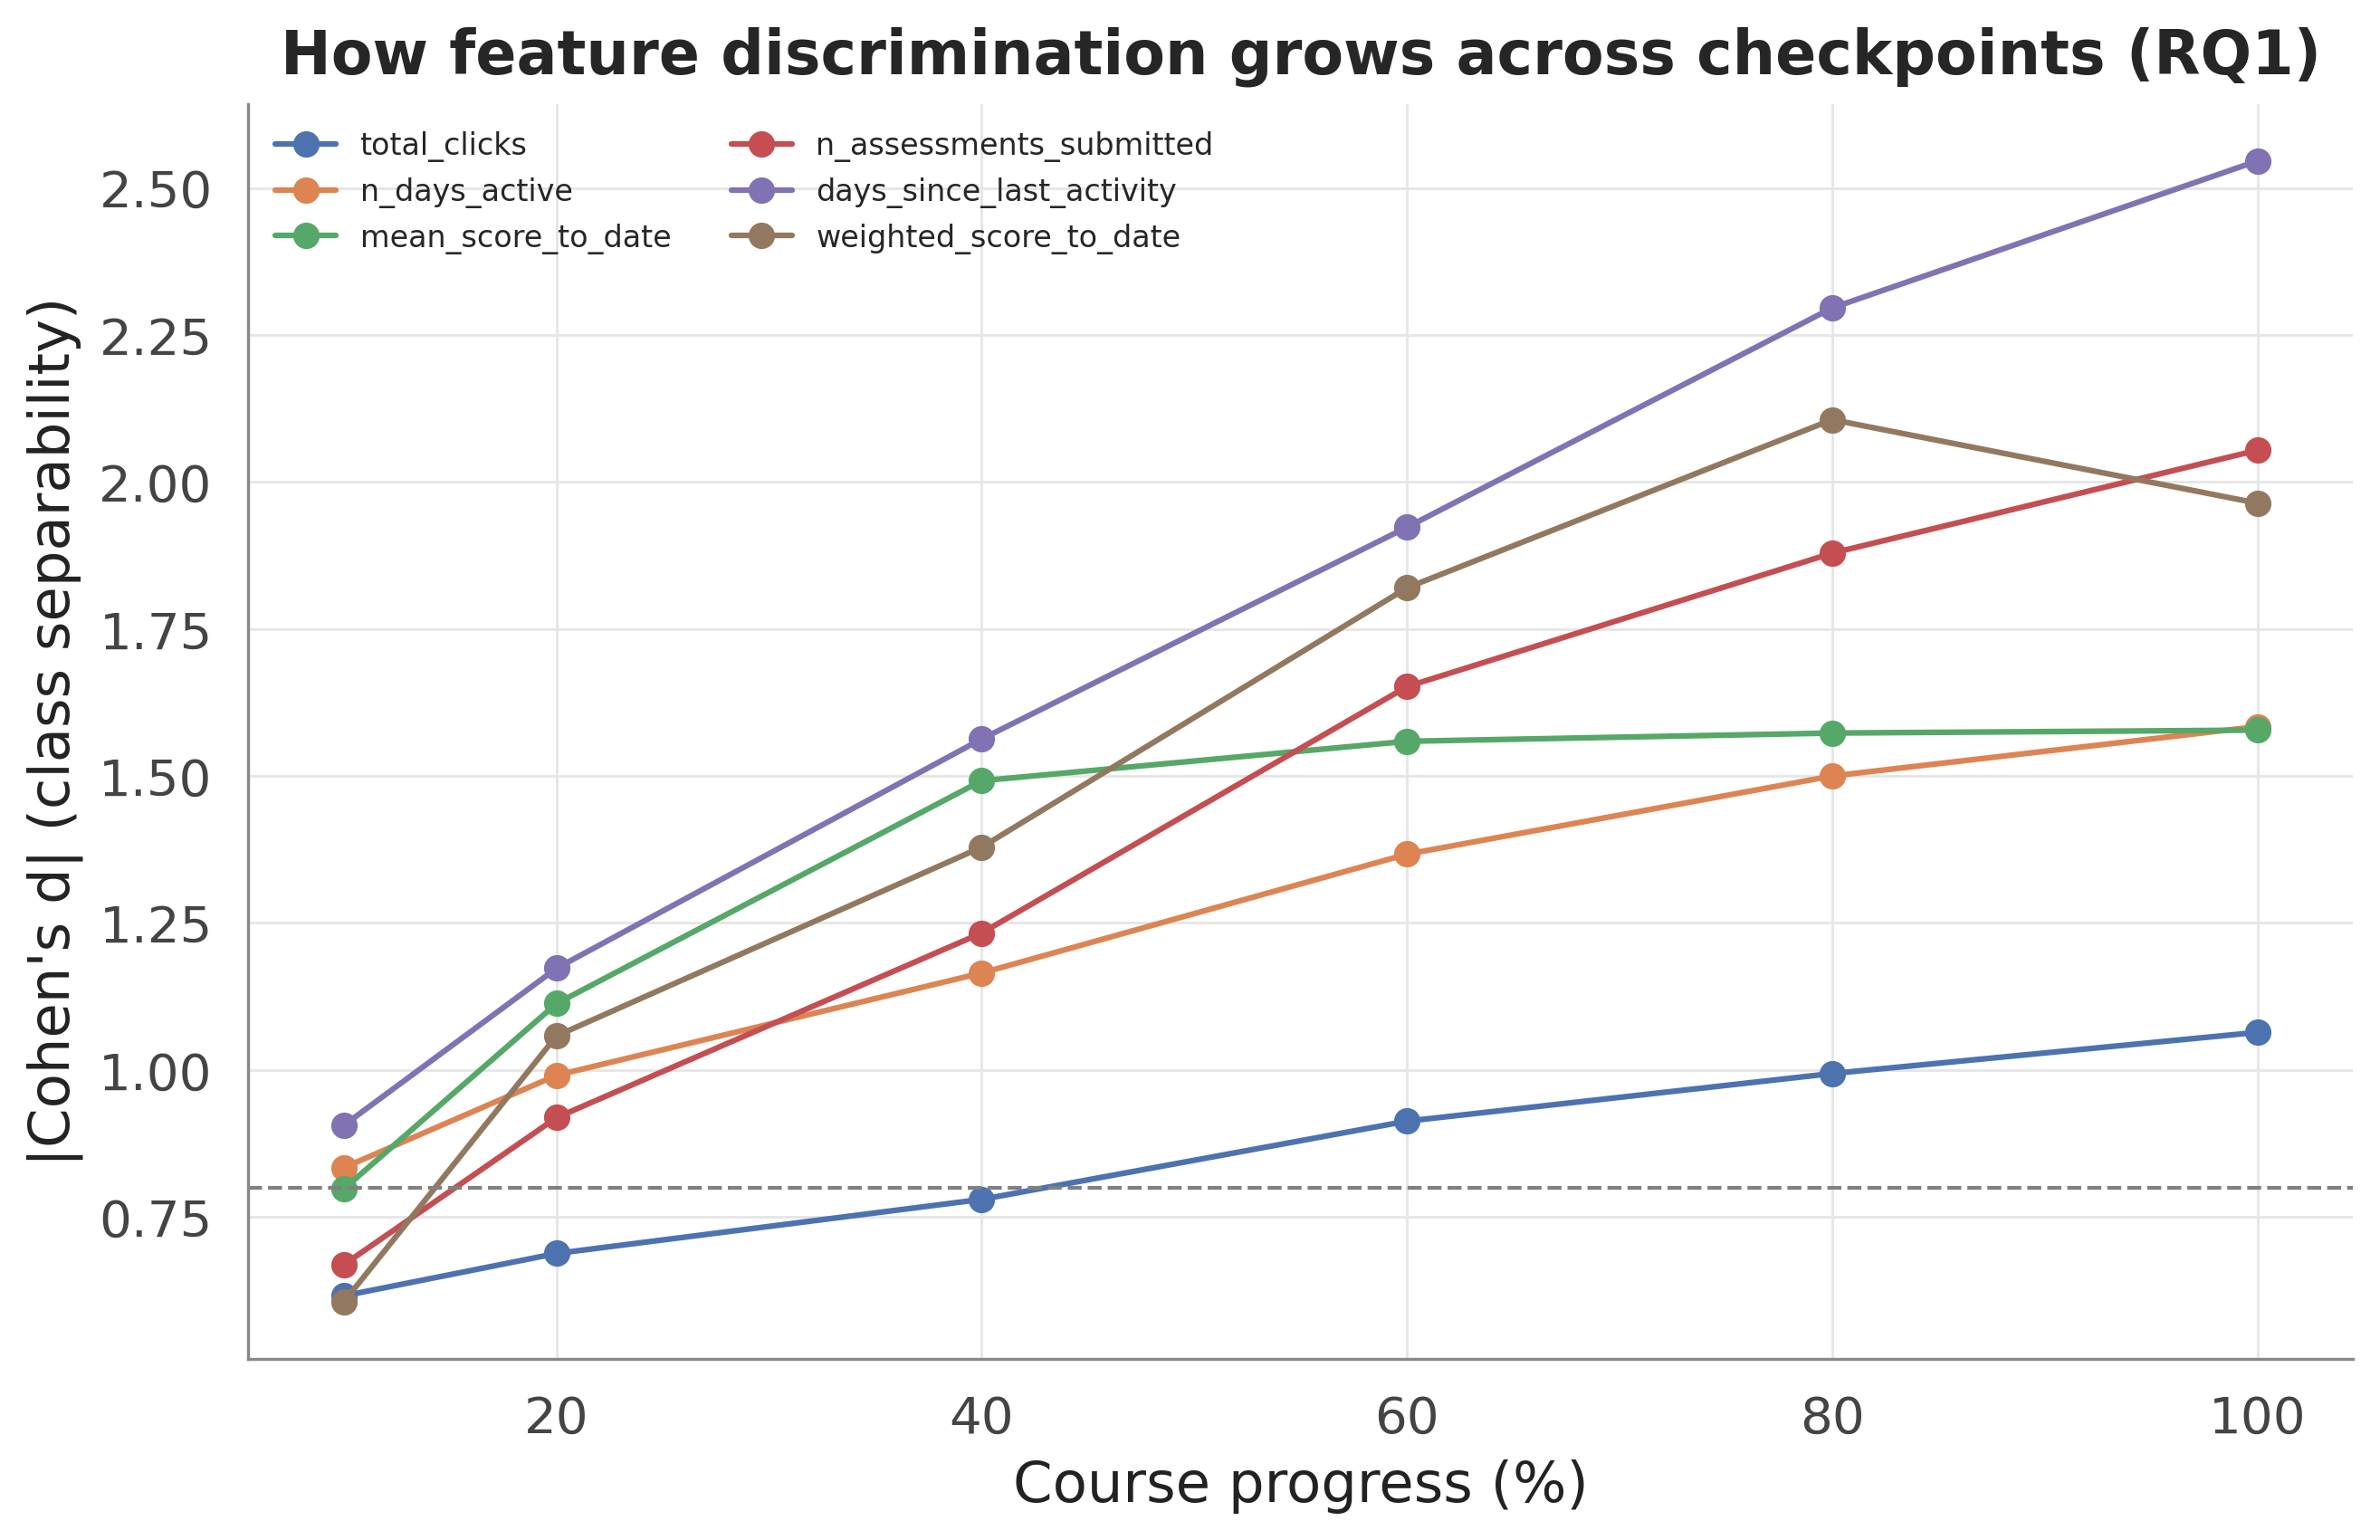
\includegraphics[width=\linewidth,height=0.66\textheight,keepaspectratio]{time_discrimination_curve.png}\\
      {\scriptsize\itshape Project figure: \tcode{reports/figures/time\_discrimination\_curve.png}}
    \end{column}
  \end{columns}
\end{frame}

% =====================================================================
\section{Exploratory Data Analysis (EDA)}
% =====================================================================

\begin{frame}{EDA Roadmap}
  \centering
  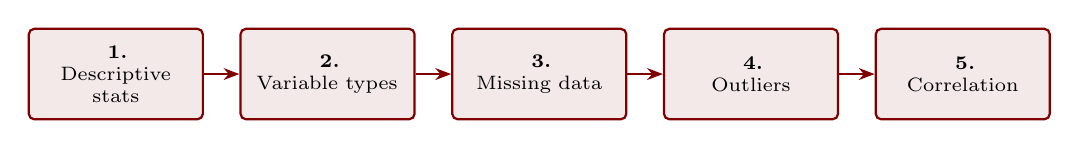
\begin{tikzpicture}[
    ebox/.style={draw=themecol,line width=0.8pt,rounded corners=2pt,fill=rowtint,
      text width=2.0cm,align=center,font=\scriptsize,inner sep=3pt,minimum height=1.15cm},
    arr/.style={-{Stealth[length=2mm]},themecol,line width=0.8pt}]
    \node[ebox](a){\textbf{1.}\\Descriptive stats};
    \node[ebox,right=0.45cm of a](b){\textbf{2.}\\Variable types};
    \node[ebox,right=0.45cm of b](c){\textbf{3.}\\Missing data};
    \node[ebox,right=0.45cm of c](d){\textbf{4.}\\Outliers};
    \node[ebox,right=0.45cm of d](e){\textbf{5.}\\Correlation};
    \draw[arr](a)--(b);\draw[arr](b)--(c);\draw[arr](c)--(d);\draw[arr](d)--(e);
  \end{tikzpicture}
  \vspace{0.5cm}\par
  \footnotesize We explore at three levels: \alert{univariate} (one variable) $\to$
  \alert{bivariate} (vs the target) $\to$ \alert{multivariate} (between variables).\\
  Raw data $\to$ patterns $\to$ conclusions that guide modelling.
\end{frame}

\begin{frame}{Descriptive Statistics (Univariate Numeric)}
  {\scriptsize
  \setlength{\tabcolsep}{5pt}\renewcommand{\arraystretch}{1.25}
  \begin{tabularx}{\textwidth}{@{}>{\ttfamily}l r r r r r r@{}}
    \toprule
    \rowcolor{themecol}\hc{Feature} & \hc{Mean} & \hc{Median} & \hc{Std} & \hc{Min} & \hc{Max} & \hc{Skew}\\
    \midrule
    total\_clicks             & 1215.1 & 602.0 & 1692.6 & 0 & 24,139 & 3.03\\
    \rowcolor{rowtint}
    n\_days\_active           & 55.5 & 40.0 & 54.5 & 0 & 286 & 1.18\\
    days\_since\_last\_activity & 97.0 & 34.0 & 100.6 & 0 & 292 & 0.57\\
    \rowcolor{rowtint}
    mean\_score\_to\_date      & 57.0 & 70.2 & 33.3 & 0 & 100 & $-$0.85\\
    weighted\_score\_to\_date  & 48.0 & 39.5 & 49.3 & 0 & 200 & 0.86\\
    \rowcolor{rowtint}
    n\_assessments\_submitted  & 5.3 & 5.0 & 4.3 & 0 & 14 & 0.28\\
    studied\_credits          & 79.8 & 60.0 & 41.1 & 30 & 655 & 1.88\\
    \rowcolor{rowtint}
    max\_clicks\_single\_day   & 109.9 & 74.0 & 142.9 & 0 & 6,988 & 10.56\\
    \bottomrule
  \end{tabularx}}
  \takeaway{Mean $\gg$ median for clickstream (total\_clicks 1215 vs 602) $\Rightarrow$ \alert{right-skew}; for \tcode{mean\_score} median $>$ mean $\Rightarrow$ left-skew. Std $\approx$ or $>$ mean $\Rightarrow$ high dispersion.}
\end{frame}

\begin{frame}{Univariate: Distributions (Histogram + KDE)}
  \centering
  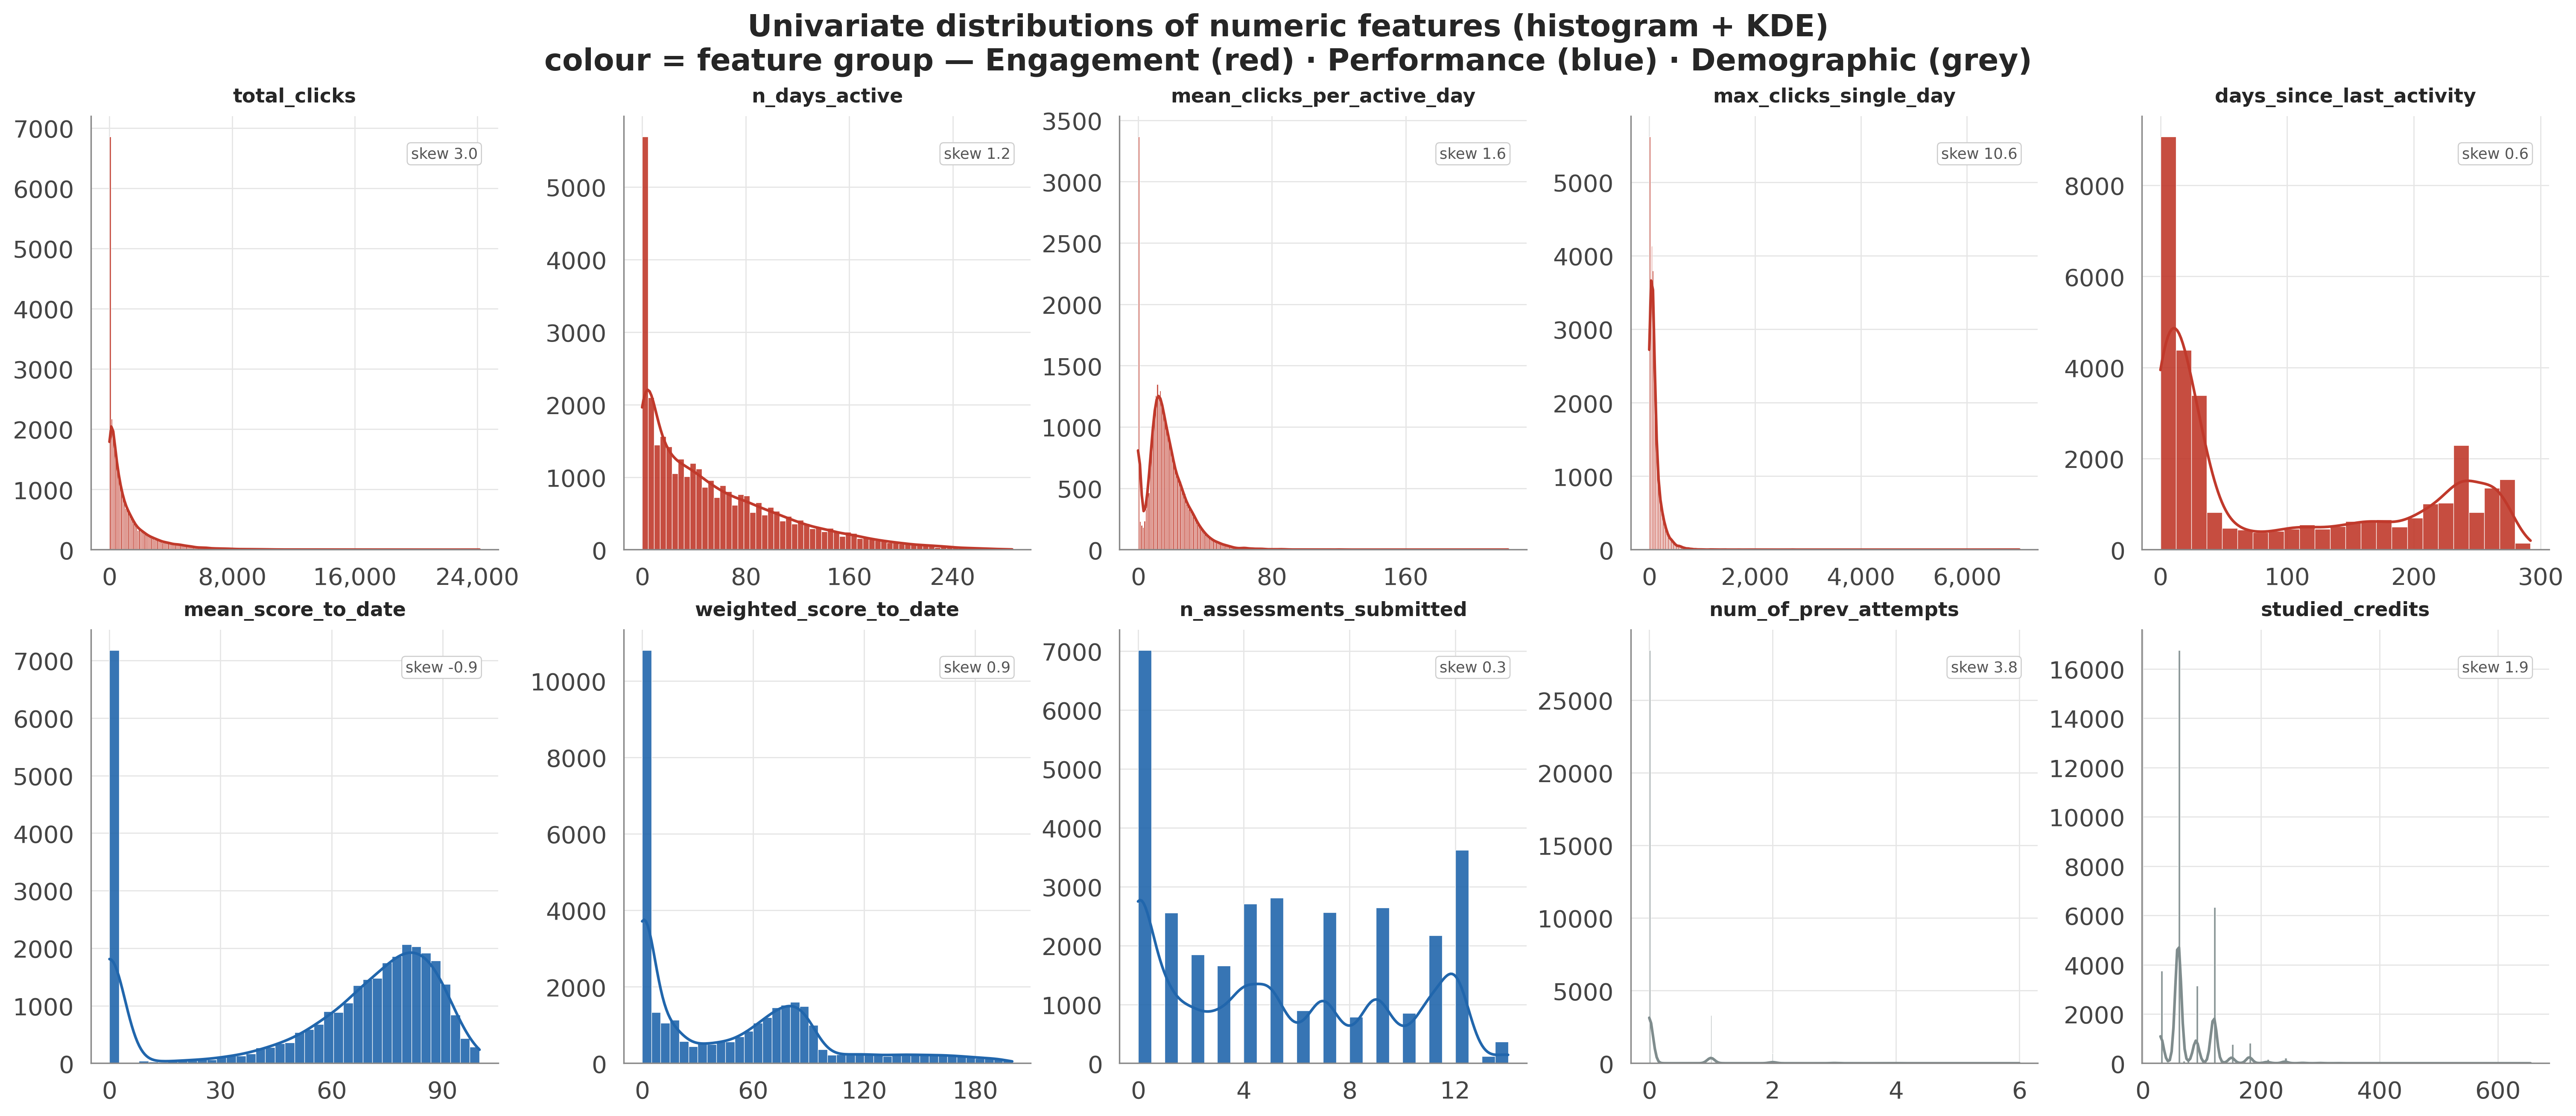
\includegraphics[width=\linewidth,height=0.74\textheight,keepaspectratio]{univariate_hist_kde.png}\\
  {\scriptsize\itshape Project figure \tcode{reports/figures/univariate\_hist\_kde.png}: clickstream right-skewed, scores bounded, \tcode{days\_idle} bimodal.}
\end{frame}

\begin{frame}{Univariate: Numeric Distributions (Box Plots)}
  \begin{columns}[T]
    \begin{column}{0.56\textwidth}
      \centering
      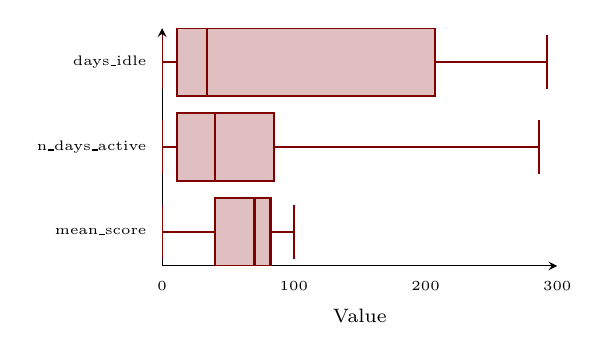
\begin{tikzpicture}
        \begin{axis}[
          width=6.6cm,height=4.6cm,
          boxplot/draw direction=x,
          xmin=0,xmax=300,xtick={0,100,200,300},xticklabel style={font=\tiny},
          ytick={1,2,3},yticklabels={mean\_score,n\_days\_active,days\_idle},
          yticklabel style={font=\tiny},
          xlabel={\scriptsize Value},axis lines=left,tick style={draw=none},
        ]
        \addplot+[boxplot prepared={lower whisker=0,lower quartile=40,median=70.2,upper quartile=82.25,upper whisker=100},fill=themecol!25,draw=themecol,solid,thick] coordinates {};
        \addplot+[boxplot prepared={lower whisker=0,lower quartile=11,median=40,upper quartile=85,upper whisker=286},fill=themecol!25,draw=themecol,solid,thick] coordinates {};
        \addplot+[boxplot prepared={lower whisker=0,lower quartile=11,median=34,upper quartile=207,upper whisker=292},fill=themecol!25,draw=themecol,solid,thick] coordinates {};
        \end{axis}
      \end{tikzpicture}
    \end{column}
    \begin{column}{0.44\textwidth}
      \footnotesize\textbf{Reading the boxes}
      \begin{itemize}\setlength\itemsep{0.3em}
        \item \tcode{mean\_score}: tight box, median (70) near upper quartile $\Rightarrow$ left-skew.
        \item \tcode{n\_days\_active}: wide, right-skewed spread.
        \item \tcode{days\_idle}: \alert{huge IQR} (11$\to$207) $\Rightarrow$ \alert{bimodal} -- active vs withdrawn students.
      \end{itemize}
      \takeaway{\scriptsize Bimodal idle-time is the clearest early-warning structure in the data.}
    \end{column}
  \end{columns}
\end{frame}

\begin{frame}{Univariate: Categorical Frequency (Highest Education)}
  \begin{columns}[T]
    \begin{column}{0.58\textwidth}
      \centering
      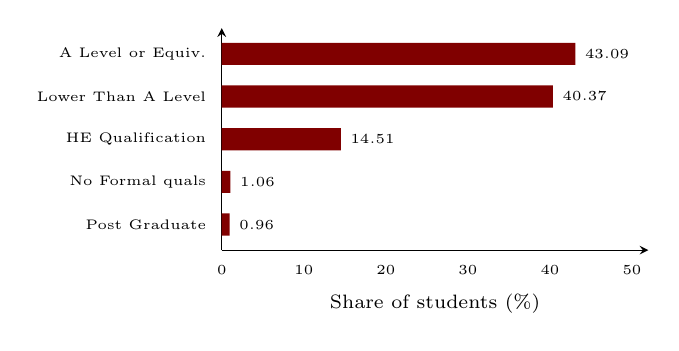
\begin{tikzpicture}
        \begin{axis}[
          width=7.0cm,height=4.4cm,
          xbar,xmin=0,xmax=52,bar width=8pt,ymin=0.4,ymax=5.6,
          ytick={1,2,3,4,5},yticklabel style={font=\tiny},
          yticklabels={Post Graduate,No Formal quals,HE Qualification,Lower Than A Level,A Level or Equiv.},
          nodes near coords,every node near coord/.append style={font=\tiny},
          xtick={0,10,20,30,40,50},xticklabel style={font=\tiny},
          xlabel={\scriptsize Share of students (\%)},axis lines=left,tick style={draw=none},
        ]
        \addplot[fill=themecol,draw=none] coordinates {(0.96,1)(1.06,2)(14.51,3)(40.37,4)(43.09,5)};
        \end{axis}
      \end{tikzpicture}
    \end{column}
    \begin{column}{0.42\textwidth}
      \footnotesize\textbf{Frequency insight}
      \begin{itemize}\setlength\itemsep{0.3em}
        \item \alert{83\%} have A-Level or below.
        \item Post-Graduate \& No-Formal are \alert{rare} ($<$1.1\% each).
        \item Rare levels $\Rightarrow$ one-hot with \tcode{handle\_unknown=ignore}, not dropping.
      \end{itemize}
      \takeaway{\scriptsize Imbalanced categoricals shape the encoding choice.}
    \end{column}
  \end{columns}
\end{frame}

\begin{frame}{Bivariate: Numeric Features vs At-Risk (Cohen's $d$)}
  \begin{columns}[T]
    \begin{column}{0.52\textwidth}
      \centering
      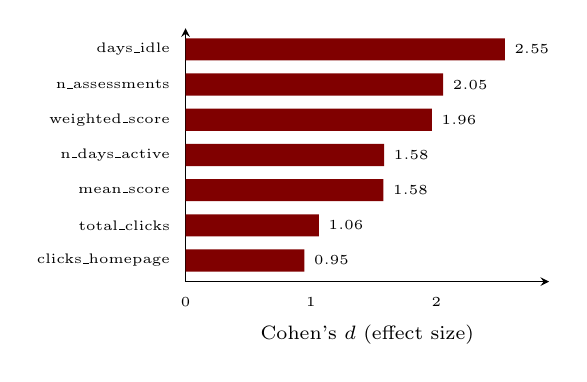
\begin{tikzpicture}
        \begin{axis}[
          width=6.2cm,height=4.8cm,
          xbar,xmin=0,xmax=2.9,bar width=8pt,ymin=0.4,ymax=7.6,
          ytick={1,2,3,4,5,6,7},yticklabel style={font=\tiny},
          yticklabels={clicks\_homepage,total\_clicks,mean\_score,n\_days\_active,weighted\_score,n\_assessments,days\_idle},
          nodes near coords,every node near coord/.append style={font=\tiny},
          xtick={0,1,2},xticklabel style={font=\tiny},
          xlabel={\scriptsize Cohen's $d$ (effect size)},
          axis lines=left,tick style={draw=none},
        ]
        \addplot[fill=themecol,draw=none] coordinates {
          (0.948,1) (1.064,2) (1.578,3) (1.584,4) (1.964,5) (2.054,6) (2.546,7)};
        \end{axis}
      \end{tikzpicture}
    \end{column}
    \begin{column}{0.48\textwidth}
      {\scriptsize
      \setlength{\tabcolsep}{3pt}\renewcommand{\arraystretch}{1.2}
      \begin{tabularx}{\textwidth}{@{}>{\ttfamily}l r r@{}}
        \toprule
        \rowcolor{themecol}\hc{Feature} & \hc{not-risk} & \hc{at-risk}\\
        \midrule
        days\_since\_last\_act & 14.2 & \textbf{171.1}\\
        \rowcolor{rowtint}
        n\_assessments        & 8.56 & \textbf{2.34}\\
        weighted\_score       & 84.9 & \textbf{15.1}\\
        \rowcolor{rowtint}
        n\_days\_active        & 91.6 & \textbf{23.2}\\
        mean\_score           & 78.5 & \textbf{37.8}\\
        \bottomrule
      \end{tabularx}}
      \takeaway{\scriptsize All \textbf{19} numeric tests significant ($q<0.05$). Behaviour, not demographics, drives risk.}
    \end{column}
  \end{columns}
\end{frame}

\begin{frame}{Multivariate: Correlation \& Multicollinearity}
  \begin{columns}[T]
    \begin{column}{0.56\textwidth}
      \centering
      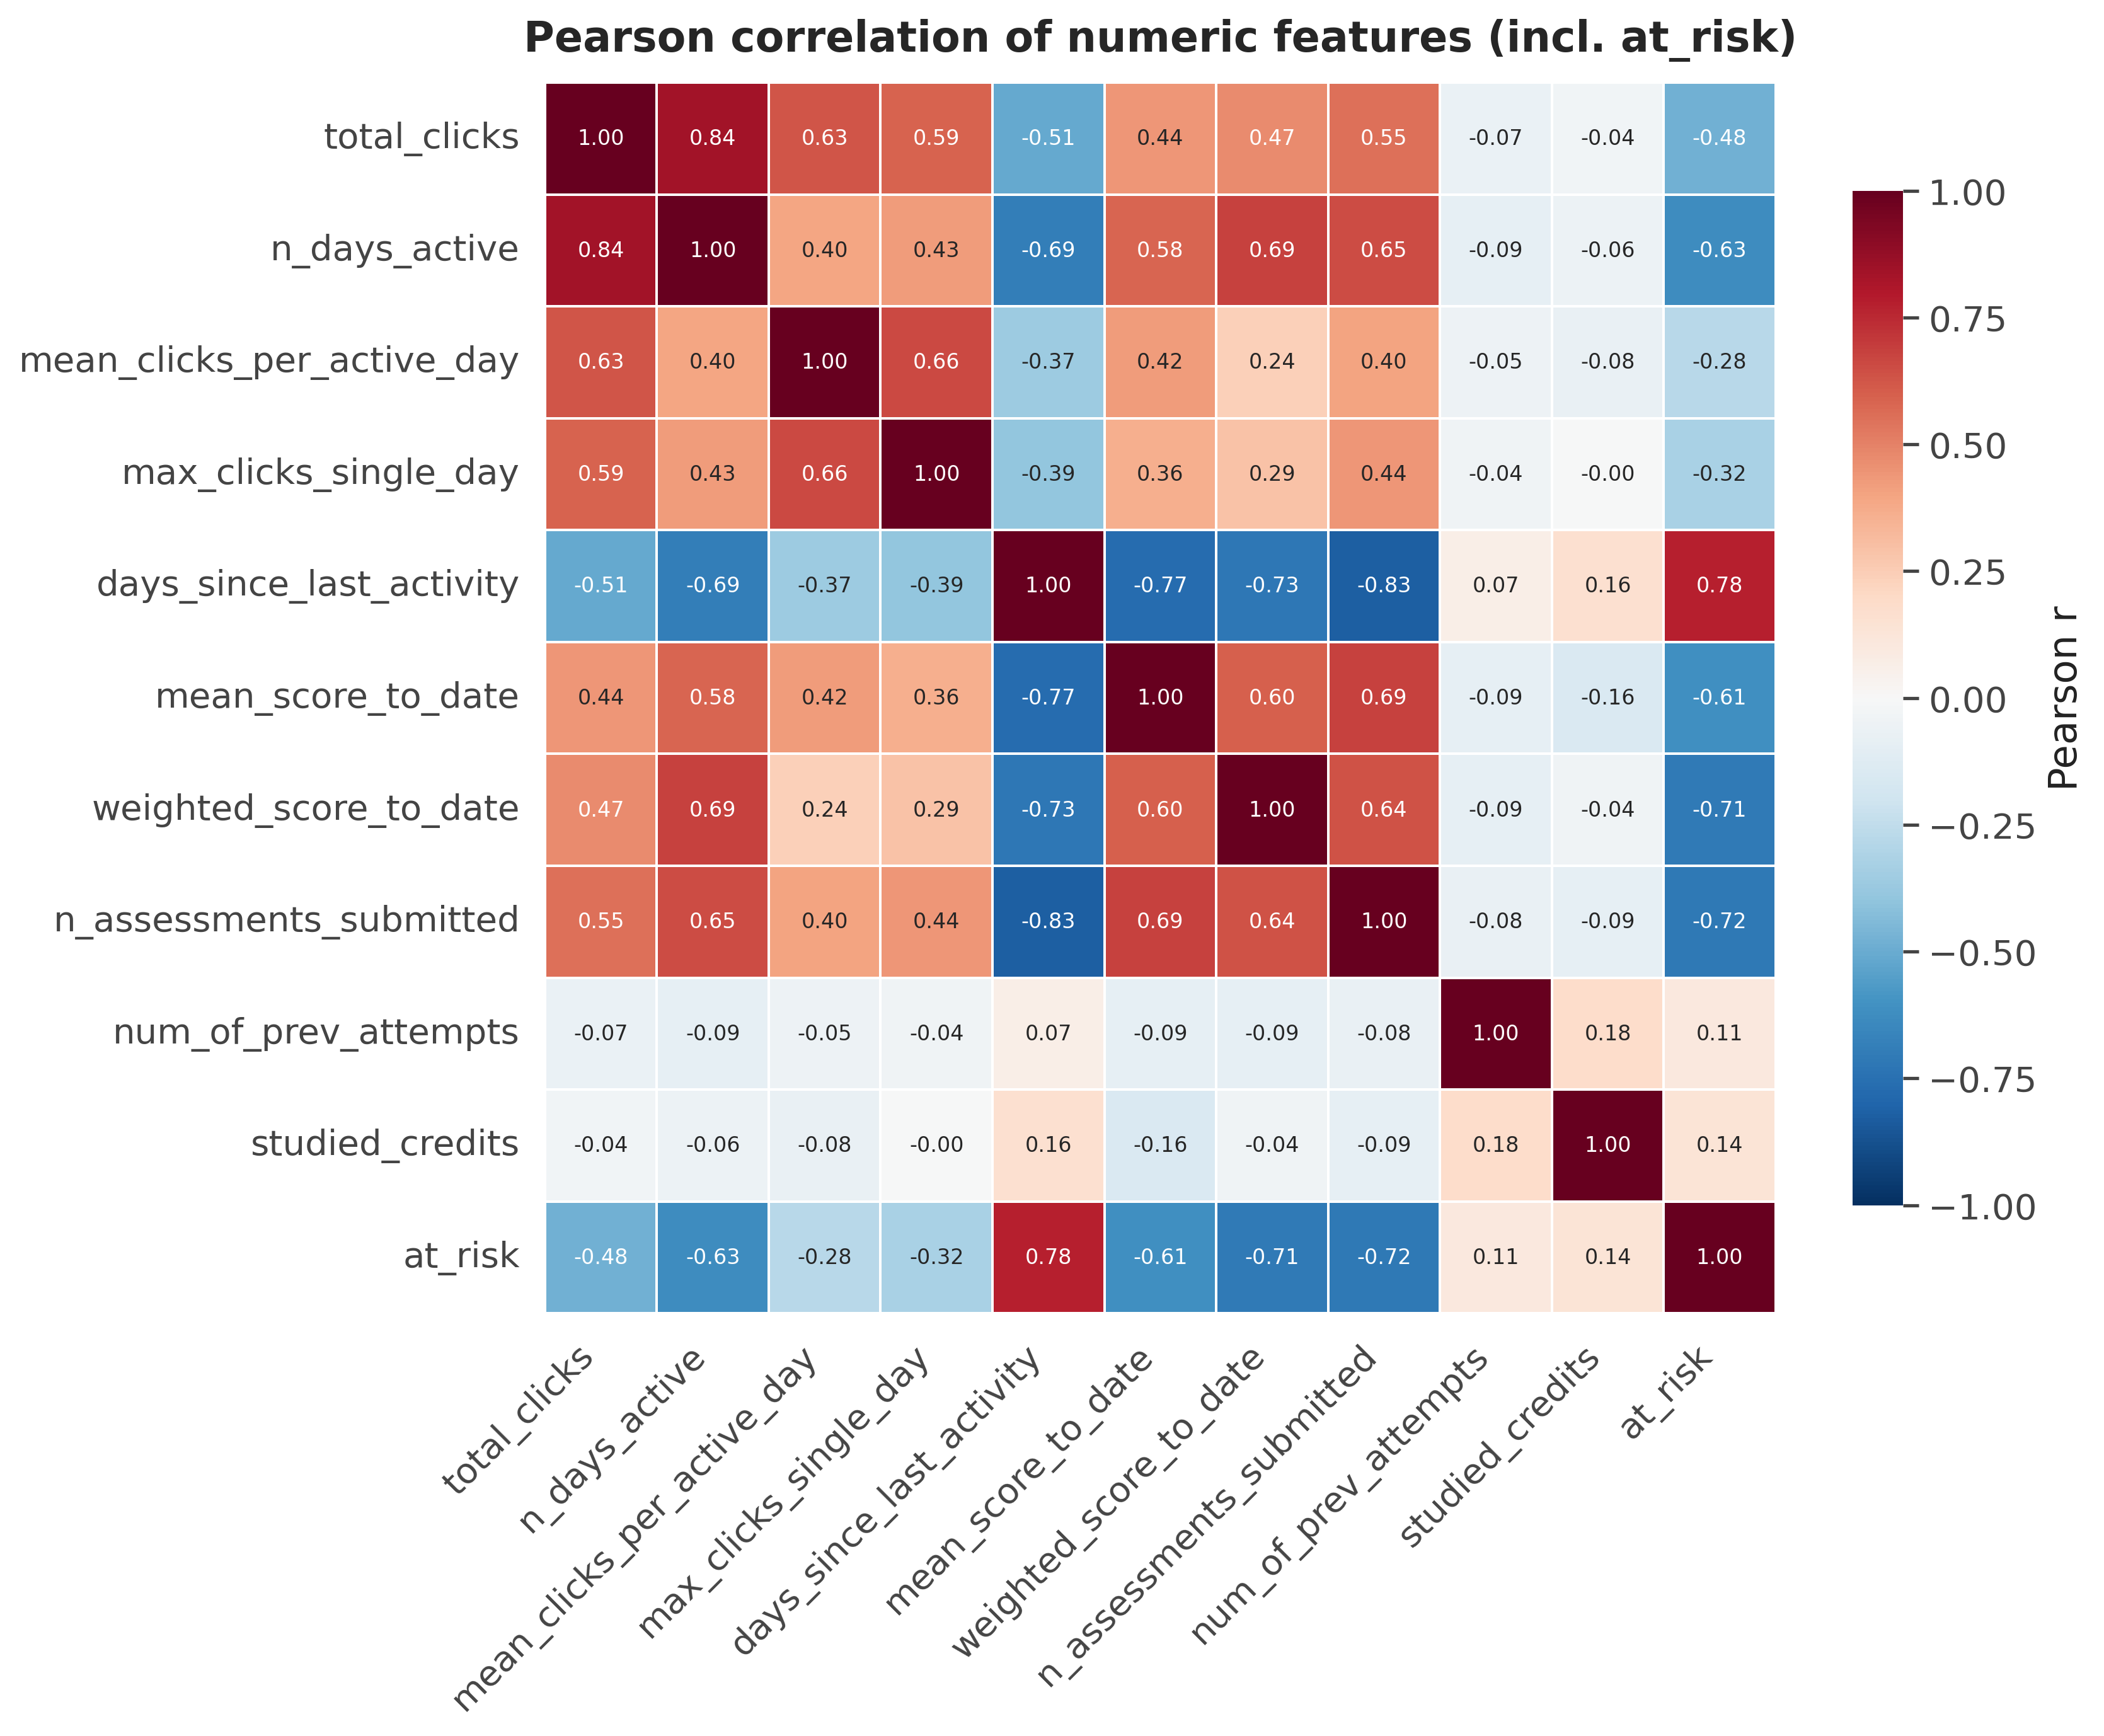
\includegraphics[width=\linewidth,height=0.68\textheight,keepaspectratio]{corr_pearson.png}\\
      {\scriptsize\itshape Project figure: \tcode{reports/figures/corr\_pearson.png}}
    \end{column}
    \begin{column}{0.44\textwidth}
      \footnotesize\textbf{Top $|r|$ with \tcode{at\_risk}}
      \begin{itemize}\setlength\itemsep{0.2em}
        \item \tcode{days\_idle} \alert{+0.78}; \tcode{n\_assessments} $-$0.72; \tcode{weighted\_score} $-$0.71.
      \end{itemize}
      \textbf{Multicollinear ($|r|\geq0.8$)}
      \begin{itemize}\setlength\itemsep{0.2em}
        \item \tcode{n\_days\_active}$\sim$\tcode{total\_clicks}: \alert{0.84}
        \item \tcode{days\_idle}$\sim$\tcode{n\_assessments}: \alert{$-$0.83}
      \end{itemize}
      \takeaway{\scriptsize No pair $\geq0.95$ $\Rightarrow$ \textbf{no leakage}. Redundancy flagged for SHAP attribution.}
    \end{column}
  \end{columns}
\end{frame}

\begin{frame}{Bivariate: Demographic Factors (Cramer's V)}
  \begin{columns}[T]
    \begin{column}{0.50\textwidth}
      {\scriptsize
      \setlength{\tabcolsep}{4pt}\renewcommand{\arraystretch}{1.25}
      \begin{tabularx}{\textwidth}{@{}>{\ttfamily}l r r@{}}
        \toprule
        \rowcolor{themecol}\hc{Factor} & \hc{Cramer's V} & \hc{$\chi^2$ $p$}\\
        \midrule
        highest\_education & \textbf{0.150} & $<10^{-157}$\\
        \rowcolor{rowtint}
        imd\_band          & \textbf{0.149} & $<10^{-147}$\\
        region             & 0.081 & $<10^{-38}$\\
        \rowcolor{rowtint}
        age\_band          & 0.069 & $<10^{-33}$\\
        disability         & 0.059 & $<10^{-26}$\\
        \rowcolor{rowtint}
        gender             & 0.022 & $5\times10^{-5}$\\
        \bottomrule
      \end{tabularx}}
    \end{column}
    \begin{column}{0.50\textwidth}
      \footnotesize\textbf{Reading it}
      \begin{itemize}\setlength\itemsep{0.3em}
        \item All significant, but associations are \alert{weak} (V $\leq$ 0.15).
        \item Strongest: \textbf{education} \& \textbf{deprivation} (imd\_band).
        \item \textbf{gender} V$=$0.022 -- practically negligible.
        \item Cohort skew: age 0--35 \textbf{70\%}; disability \textbf{9.7\%}.
      \end{itemize}
      \takeaway{\scriptsize Demographic effect ($V\!\leq\!0.15$) $\ll$ behavioural effect ($d$ up to \textbf{2.5}) -- watch fairness on imd/education, not gender.}
    \end{column}
  \end{columns}
\end{frame}

\begin{frame}{Temporal Pattern -- the ``Withdrawn'' Signal}
  \begin{columns}[T]
    \begin{column}{0.50\textwidth}
      \centering
      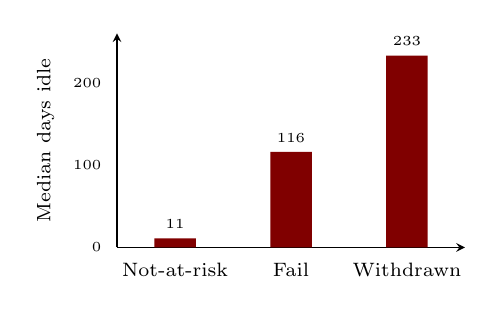
\begin{tikzpicture}
        \begin{axis}[
          width=6.0cm,height=4.3cm,
          ybar,ymin=0,ymax=260,bar width=15pt,
          symbolic x coords={Not-at-risk,Fail,Withdrawn},
          xtick=data,xticklabel style={font=\scriptsize},
          nodes near coords,every node near coord/.append style={font=\tiny},
          ylabel={\scriptsize Median days idle},yticklabel style={font=\tiny},
          axis lines=left,tick style={draw=none},enlarge x limits=0.25,
        ]
        \addplot[fill=themecol,draw=none] coordinates {(Not-at-risk,11)(Fail,116)(Withdrawn,233)};
        \end{axis}
      \end{tikzpicture}
    \end{column}
    \begin{column}{0.50\textwidth}
      \footnotesize\textbf{Median activity by outcome}
      {\scriptsize
      \setlength{\tabcolsep}{5pt}\renewcommand{\arraystretch}{1.25}
      \begin{tabularx}{\textwidth}{@{}l r r@{}}
        \toprule
        \rowcolor{themecol}\hc{Outcome} & \hc{Days idle} & \hc{Total clicks}\\
        \midrule
        Not-at-risk & 11  & 1,425\\
        \rowcolor{rowtint}
        Fail        & 116 & 317\\
        Withdrawn   & \textbf{233} & \textbf{89}\\
        \bottomrule
      \end{tabularx}}
      \takeaway{\scriptsize Withdrawn $\approx$ near-zero engagement $\Rightarrow$ trivially separable at \emph{late} checkpoints. Recall/PR-AUC can look \textbf{optimistic} late -- the documented Option-A limitation; the hard test is the \textbf{early} checkpoints.}
    \end{column}
  \end{columns}
\end{frame}

\begin{frame}{EDA -- Key Findings}
  \footnotesize
  \begin{itemize}\setlength\itemsep{0.5em}
    \item \textbf{Distributions:} clickstream features are strongly right-skewed (skew up to \alert{34.7}) $\Rightarrow$ log1p; scores are bounded / left-skewed.
    \item \textbf{Univariate:} \tcode{days\_idle} is \alert{bimodal} -- the structural signature of disengagement.
    \item \textbf{Bivariate (numeric):} engagement \& performance separate at-risk strongly (Cohen's $d$ up to \alert{2.55}); all 19 features significant.
    \item \textbf{Bivariate (categorical):} demographic association is weak (Cramer's V $\leq$ 0.15) -- behaviour dominates.
    \item \textbf{Multivariate:} 2 multicollinear pairs ($|r|\geq0.8$); none $\geq0.95$ $\Rightarrow$ no leakage suspect.
    \item \textbf{Hypothesis for modelling:} recent inactivity + few submissions are the earliest reliable risk markers.
  \end{itemize}
\end{frame}

% =====================================================================
\section*{Wrap-up}
% =====================================================================

\begin{frame}{Summary}
  \footnotesize
  \begin{enumerate}\setlength\itemsep{0.5em}
    \item[\alert{\textbf{01}}] \textbf{Required data} -- 7 OULAD tables, grain \tcode{(student,module,presentation)}; 32,593 rows, at-risk 52.8\%.
    \item[\alert{\textbf{02}}] \textbf{Collection} -- public CC-BY 4.0 secondary data; anonymised; same as base studies.
    \item[\alert{\textbf{03}}] \textbf{Cleaning} -- 0 duplicates; missing by mechanism (MAR/MNAR/structural); skew up to 34.7 $\to$ log1p/winsorise; no row dropped.
    \item[\alert{\textbf{04}}] \textbf{Transformation} -- 28 features, 5 types $\to$ 49-col dense matrix; fit on train only.
    \item[\alert{\textbf{05}}] \textbf{Split \& leakage} -- 20\% hold-out + 5$\times$5 CV; time-aware cuts; 19/19 tests pass.
    \item[\alert{\textbf{06}}] \textbf{Analysis} -- behaviour dominates (\tcode{days\_idle} $d=2.55$); demographics weak (V$\leq$0.15); withdrawn drives late-checkpoint optimism.
  \end{enumerate}
\end{frame}

\begin{frame}{Thank you}
  \vfill\centering
  {\Huge \alert{Thank you}}\\[1.0em]
  {\footnotesize\textbf{Key references}}\\[0.3em]
  {\scriptsize
   Kuzilek, Hlosta, Zdrahal (2017), \emph{OULAD}, Scientific Data 4:170171 -- CC-BY 4.0.\quad
   Adnan et al.\ (2021), \emph{IEEE Access} 9.\\
   Tomasevic et al.\ (2020), \emph{Computers \& Education} 143.\quad
   Chawla et al.\ (2002), \emph{SMOTE}, JAIR.}
  \vfill
\end{frame}

\end{document}
